% Image fixe de l'animation ebva-directionnelle, dans son état initial :
% direction u proportionnelle à (1,2), soit theta = 63,43°.
% f(x,y) = y^2/x : la formule du gradient donne sin(theta), la dérivée
% directionnelle vaut u_2^2/u_1 = sin^2(theta)/cos(theta) (et sin(theta) sur l'axe x = 0).
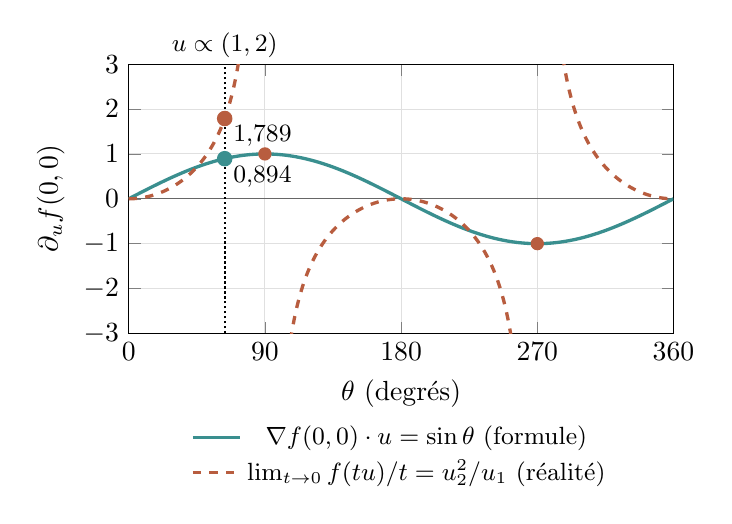
\begin{tikzpicture}
    \begin{axis}[
        width=8.5cm,
        height=5cm,
        xmin=0, xmax=360,
        ymin=-3, ymax=3,
        xtick={0,90,180,270,360},
        ytick={-3,-2,-1,0,1,2,3},
        xlabel={$\theta$ (degrés)},
        ylabel={$\partial_u f(0,0)$},
        grid=major,
        grid style={black!12},
        legend style={at={(0.5,-0.3)}, anchor=north, draw=none, font=\small},
        restrict y to domain=-4:4,
        unbounded coords=jump,
        samples=200,
        clip mode=individual,
    ]
    \draw[black!60] (axis cs:0,0) -- (axis cs:360,0);
    % Formule du gradient : (0,1).u = sin(theta)
    \addplot[very thick, color={rgb,255:red,58;green,143;blue,143}, domain=0:360] {sin(x)};
    \addlegendentry{$\nabla f(0,0)\cdot u = \sin\theta$ (formule)}
    % Dérivée directionnelle réelle : u_2^2/u_1, asymptotes en 90° et 270°
    \addplot[very thick, dashed, color={rgb,255:red,184;green,93;blue,63}, domain=0:89.5] {sin(x)^2/cos(x)};
    \addlegendentry{$\lim_{t\to0} f(tu)/t = u_2^2/u_1$ (réalité)}
    \addplot[very thick, dashed, color={rgb,255:red,184;green,93;blue,63}, domain=90.5:269.5, forget plot] {sin(x)^2/cos(x)};
    \addplot[very thick, dashed, color={rgb,255:red,184;green,93;blue,63}, domain=270.5:360, forget plot] {sin(x)^2/cos(x)};
    % Sur l'axe x = 0, f(0,t) = t : la dérivée vaut sin(theta), soit +1 et -1
    \addplot[only marks, mark=*, mark size=2.2pt, color={rgb,255:red,184;green,93;blue,63}, forget plot] coordinates {(90,1) (270,-1)};
    % Direction u proportionnelle à (1,2)
    \draw[densely dotted, thick] (axis cs:63.43,-3) -- (axis cs:63.43,3);
    \addplot[only marks, mark=*, mark size=2.6pt, color={rgb,255:red,58;green,143;blue,143}, forget plot] coordinates {(63.43,0.894)};
    \addplot[only marks, mark=*, mark size=2.6pt, color={rgb,255:red,184;green,93;blue,63}, forget plot] coordinates {(63.43,1.789)};
    \node[anchor=north west, font=\small, inner sep=1.5pt] at (axis cs:66,0.82) {$0{,}894$};
    \node[anchor=north west, font=\small, inner sep=1.5pt] at (axis cs:66,1.75) {$1{,}789$};
    % Au-dessus du cadre, au bout de la ligne : dans le cadre, les courbes la croisent
    \node[anchor=south, font=\small, inner sep=2pt] at (axis cs:63.43,3) {$u \propto (1,2)$};
    \end{axis}
\end{tikzpicture}
